
This section discusses the results presented in Section~\ref{sec:results} and their broader implications for multimodal machine learning. The key areas of focus include: \textbf{(i)} the effectiveness and flexibility of C-MAMs, \textbf{(ii)} insights from ablation studies, and \textbf{(iii)} the observed multimodal model behaviours. Additionally, we highlight the limitations of the approach and its potential future directions.

\textbf{Effectiveness of C-MAMs:} The results from \Cref{sec:results} demonstrate that C-MAMs effectively mitigate performance degradation due to missing modality data, consistently improving inference-time performance across multiple models and datasets. This performance gain is particularly significant given that C-MAMs are trained post-hoc and do not interfere with the original multimodal model. For AVMNIST, MM-IMDb, and IEMOCAP, C-MAMs improved performance by up to 39\%, 30\%, and 28\%, respectively, compared to the missing modality baseline. Even when performance did not fully return to the original multimodal model's accuracy, the improvements confirm that C-MAMs recover meaningful information for inference.

A central strength of C-MAMs lies in their \textbf{architectural simplicity} coupled with deployment flexibility. Unlike complex generative models or contrastive learning frameworks that introduce additional optimisation constraints, C-MAMs rely on association networks trained with an MSE loss to map available modality features to missing ones. This straightforward formulation proves sufficient to reconstruct embeddings that significantly enhance multimodal inference, reinforcing the argument for simple, modular solutions in real-world deployment. The modularity of C-MAMs \textbf{allows them to be trained independently of the original multimodal model's objectives}, making them particularly suitable for distributed learning environments such as federated learning or Internet of Things applications.

In practical deployments, C-MAMs offer significant advantages through their targeted reconstruction approach. Each modality is treated independently, ensuring the reconstruction process is optimised specifically for that missing modality. This design decision ensures that each reconstruction network focuses on the specific cross-modal relationships most relevant for a given modality. The ability to deploy C-MAMs selectively, only when and where they are needed, minimises computational overhead and provides flexibility in resource-constrained environments. For instance, different medical sensors across hospitals may record different modalities in a federated learning setting for smart healthcare Internet of Things. Since each hospital has different hardware capabilities and privacy constraints, not all modalities will always be available for training. Deploying C-MAMs in such an environment ensures that missing modality embeddings can be reconstructed locally, enabling robust multimodal learning without requiring centralised data collection or retraining the global model. While these results demonstrate the general effectiveness of C-MAMs, a closer examination of modality relationships across datasets reveals additional insights into the factors influencing reconstruction success.

Our results demonstrate that modality alignment is not always predictive of reconstruction success, and in some cases, contrastive information may play a role in limiting performance recovery. In MM-IMDb, the text modality successfully reconstructed the missing image modality, with final model performance nearly identical to the baseline, despite the reconstructed image embeddings exhibiting low similarity to the original features. This suggests that the success of C-MAMs is not solely dependent on feature space similarity but on whether the reconstructed modality captures the critical features necessary for the downstream task.

A similar observation arises in AVMNIST for audio-to-image reconstruction, where despite high MAE/MSE errors (Table \ref{tab:errors}), the C-MAM nearly fully recovered the baseline performance (within 0.001 of the original model). This suggests that multimodal models can tolerate deviations in reconstructed features if the information remains useful. However, performance recovery was more limited in Kinetics-Sounds, where the audio-to-video C-MAM exhibited extremely high MAE/MSE errors. While the C-MAM still improved results over missing modality baselines, the overall performance gain was lower than other datasets. Despite substantial improvements over the missing modality baseline, the relatively lower performance gains in Kinetics-Sounds suggest that audio and video may exhibit contrastive relationships in some samples. In these cases, reconstructing video features from audio may introduce inconsistent or conflicting features, limiting the overall effectiveness of C-MAMs.

Taken together, these results indicate that C-MAMs can effectively reconstruct missing modalities even when feature space similarity is low, but the extent of performance recovery depends on modality relationships, when modalities are strongly correlated, even high reconstruction errors do not necessarily hinder full recovery, such as with AVMNIST.

\textbf{Ablation Studies:}
A series of ablation studies was conducted to better understand C-MAMs' behaviour. These analyses focused on embedding alignment, reconstruction quality, statistical properties of the generated features, and the contribution of individual modalities in bimodal settings. Each study provides additional confidence in the robustness of C-MAM-generated embeddings and their impact on inference performance.

\textbf{T-SNE Visualisations:}
Figure~\ref{fig:tsne} presents t-SNE projections of C-MAM-generated embeddings compared to their ground-truth counterparts. The visualisation highlights that, despite some variance, C-MAMs generate embeddings that largely align with original modality embeddings, particularly in AVMNIST and MM-IMDb. While t-SNE does not fully capture the structural relationships within the embedding space, these results suggest that the generated features retain relevant information for inference.
% \begin{landscape}
\begin{figure}[!p]
    \centering
    \begin{subfigure}[b]{0.24\textwidth}
        \centering
        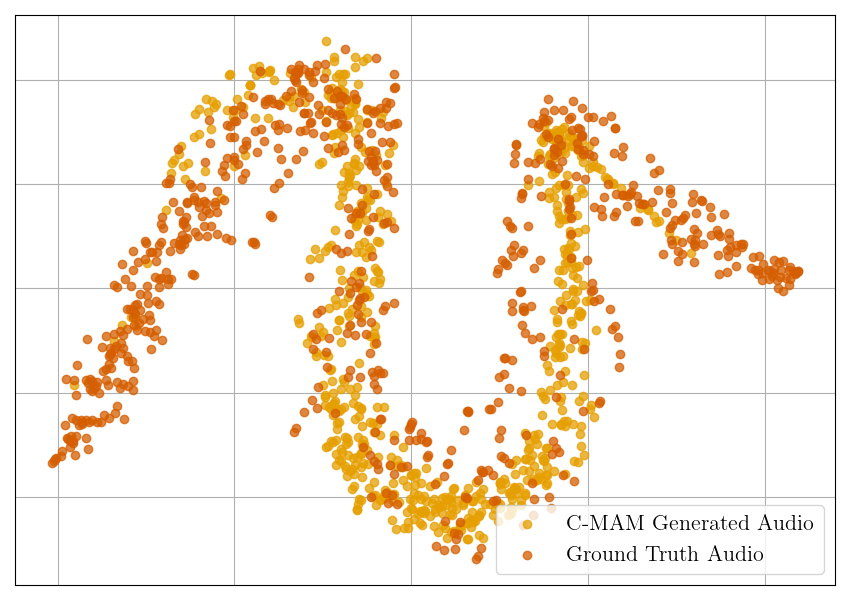
\includegraphics[width=\textwidth]{imgs/tsne/sns_audio_cmam_2.png}
        \caption*{AudioSet (V $\rightarrow$ A)}
    \end{subfigure}
    \begin{subfigure}[b]{0.24\textwidth}
        \centering
        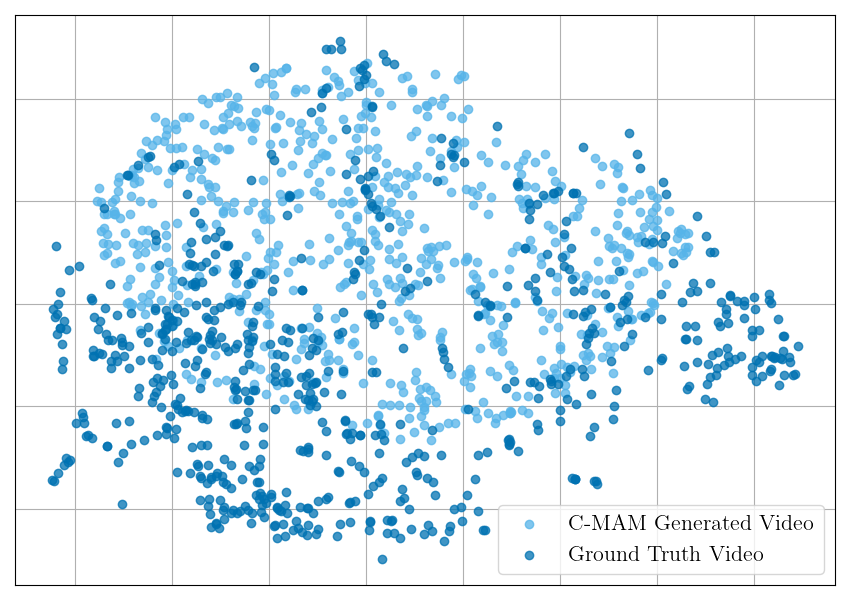
\includegraphics[width=\textwidth]{imgs/tsne/sns_video_cmam_3.png}
        \caption*{AudioSet (A $\rightarrow$ V)}
    \end{subfigure}
    \begin{subfigure}[b]{0.24\textwidth}
        \centering
        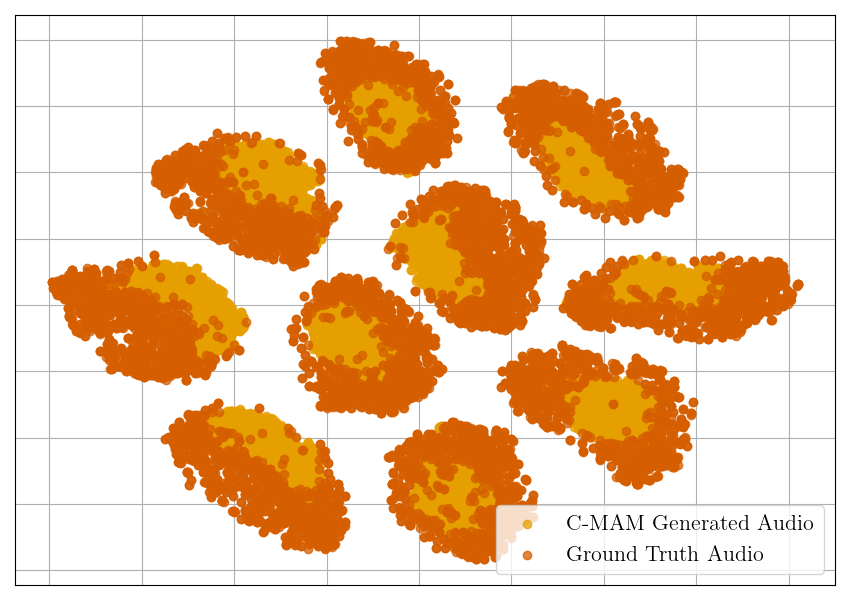
\includegraphics[width=\textwidth]{imgs/tsne/avmnist_audio_cmam_1.png}
        \caption*{AVMNIST (I $\rightarrow$ A)}
    \end{subfigure}
    \begin{subfigure}[b]{0.24\textwidth}
        \centering
        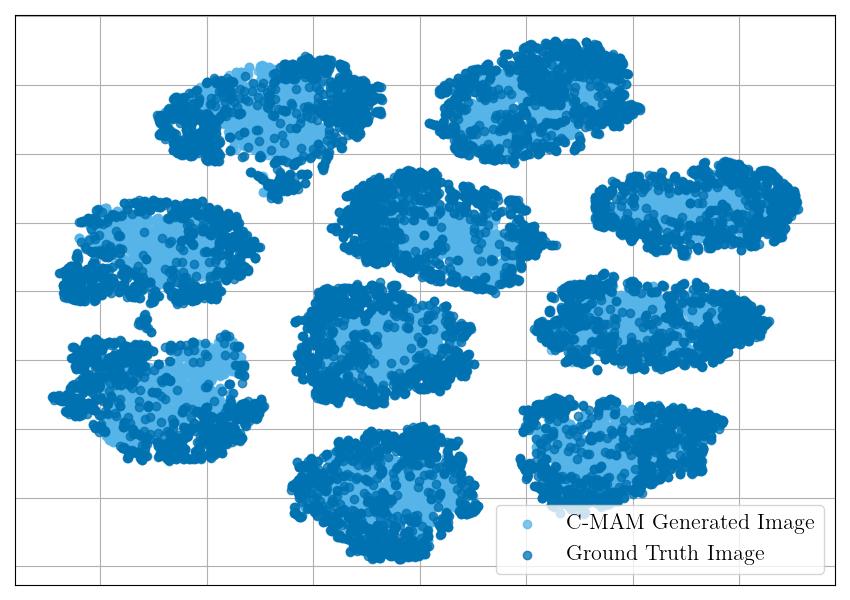
\includegraphics[width=\textwidth]{imgs/tsne/avmnist_video_cmam_1.png}
        \caption*{AVMNIST (A $\rightarrow$ I)}
    \end{subfigure}
    \centering
    \begin{subfigure}[b]{0.24\textwidth}
        \centering
        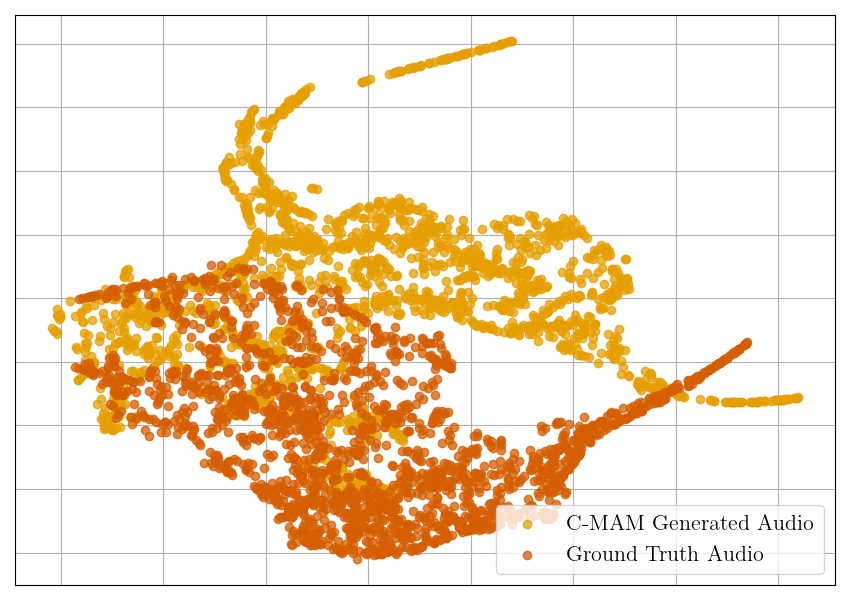
\includegraphics[width=\textwidth]{imgs/tsne/ks_audio_cmam_1.png}
        \caption*{Kinetics-Sounds (V $\rightarrow$ A)}
    \end{subfigure}
    \begin{subfigure}[b]{0.24\textwidth}
        \centering
        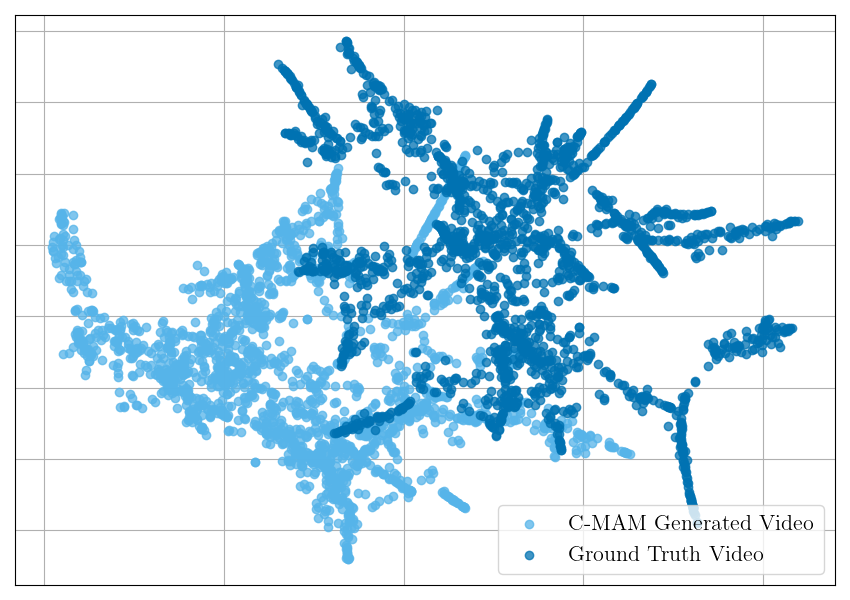
\includegraphics[width=\textwidth]{imgs/tsne/ks_video_cmam_1.png}
        \caption*{Kinetics-Sounds (A $\rightarrow$ V)}
    \end{subfigure}
    \begin{subfigure}[b]{0.24\textwidth}
        \centering
        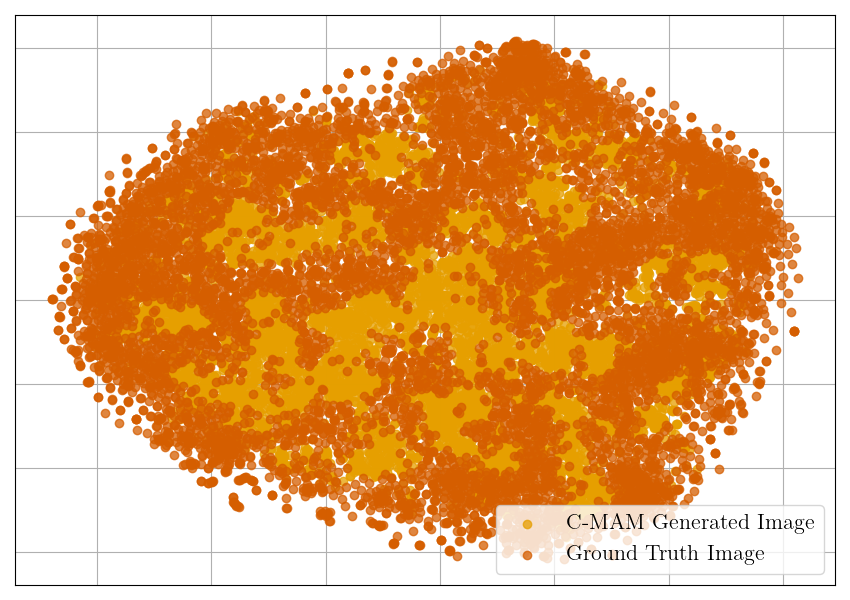
\includegraphics[width=\textwidth]{imgs/tsne/mmimdb_image_cmam_1.png}
        \caption*{MM-IMDb (T $\rightarrow$ I)}
    \end{subfigure}
    \begin{subfigure}[b]{0.24\textwidth}
        \centering
        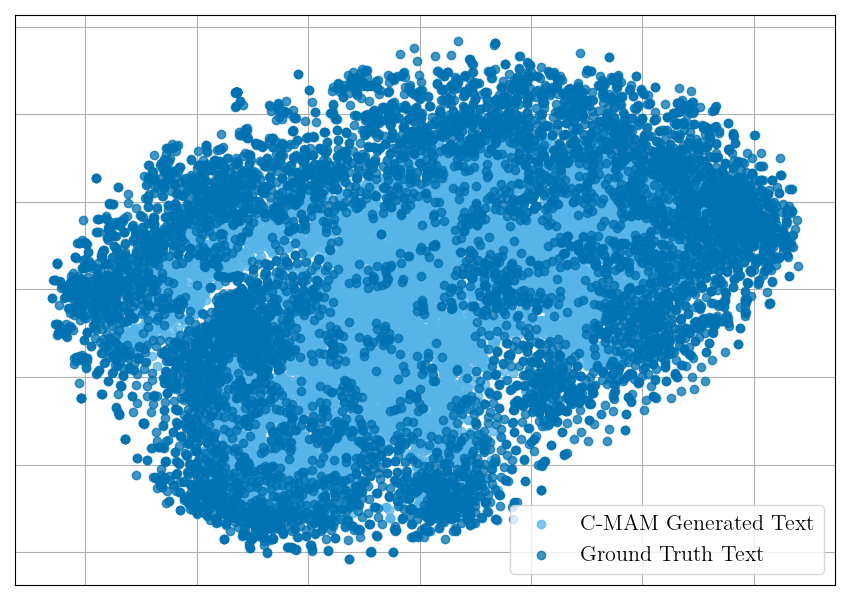
\includegraphics[width=\textwidth]{imgs/tsne/mmimdb_text_cmam_1.png}
        \caption*{MM-IMDb (I $\rightarrow$ T)}
    \end{subfigure}

    \centering

    \begin{subfigure}[b]{0.24\textwidth}
        \centering
        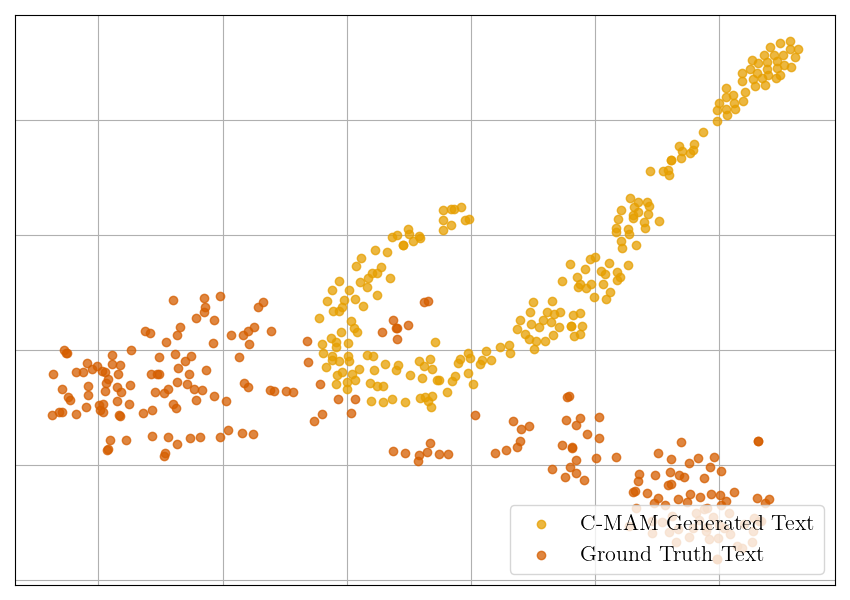
\includegraphics[width=\textwidth]{imgs/tsne/emt_dlfr_baseline_mosi_tsne.png}
        \caption*{EMT-DLFR MOSI (AV $\rightarrow$ T)}
    \end{subfigure}
    \begin{subfigure}[b]{0.24\textwidth}
        \centering
        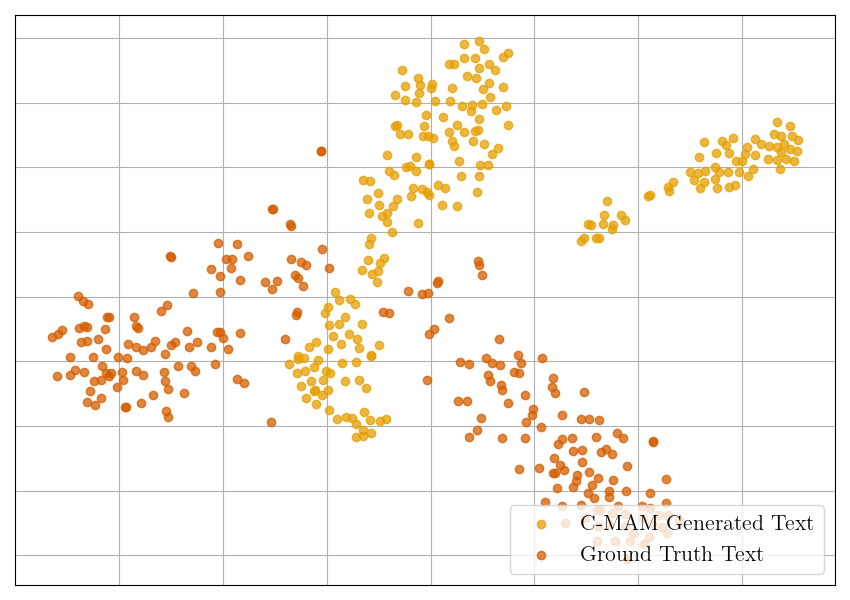
\includegraphics[width=\textwidth]{imgs/tsne/emt_dlfr_robust_baseline_mosi_tsne.png}
        \caption*{R. EMT-DLFR MOSI (AV $\rightarrow$ T)}
    \end{subfigure}
    \begin{subfigure}[b]{0.24\textwidth}
        \centering
        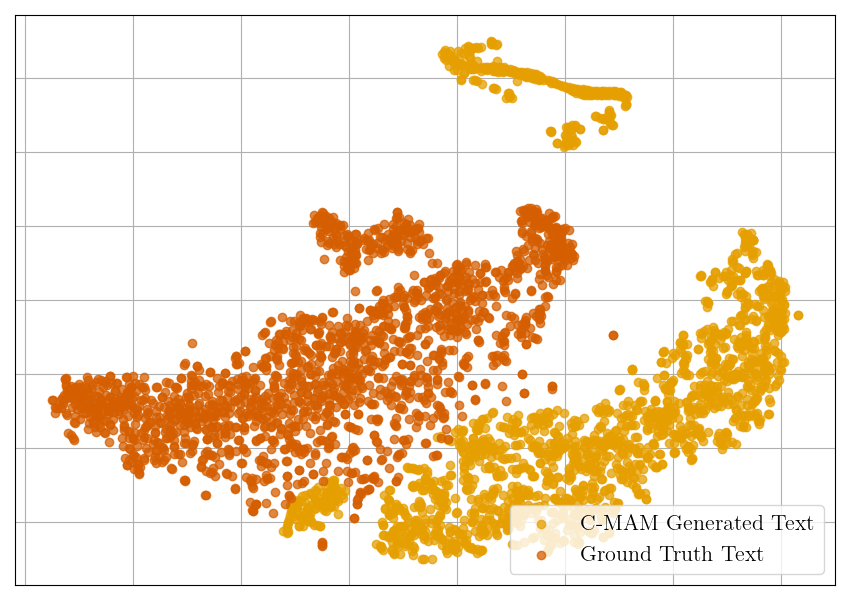
\includegraphics[width=\textwidth]{imgs/tsne/emt_dlfr_baseline_mosei_tsne.png}
        \caption*{EMT-DLFR MOSEI (AV $\rightarrow$ T)}
    \end{subfigure}
    \begin{subfigure}[b]{0.24\textwidth}
        \centering
        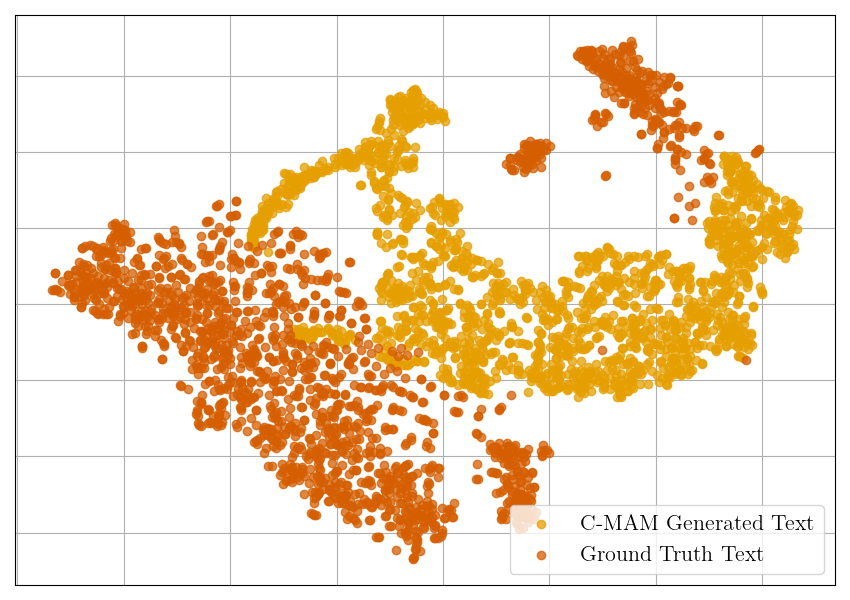
\includegraphics[width=\textwidth]{imgs/tsne/emt_dlfr_robust_baseline_mosei_tsne.png}
        \caption*{R. EMT-DLFR MOSEI (AV $\rightarrow$ T)}
    \end{subfigure}
\\
    \centering
    \begin{subfigure}[b]{0.24\textwidth}
        \centering
        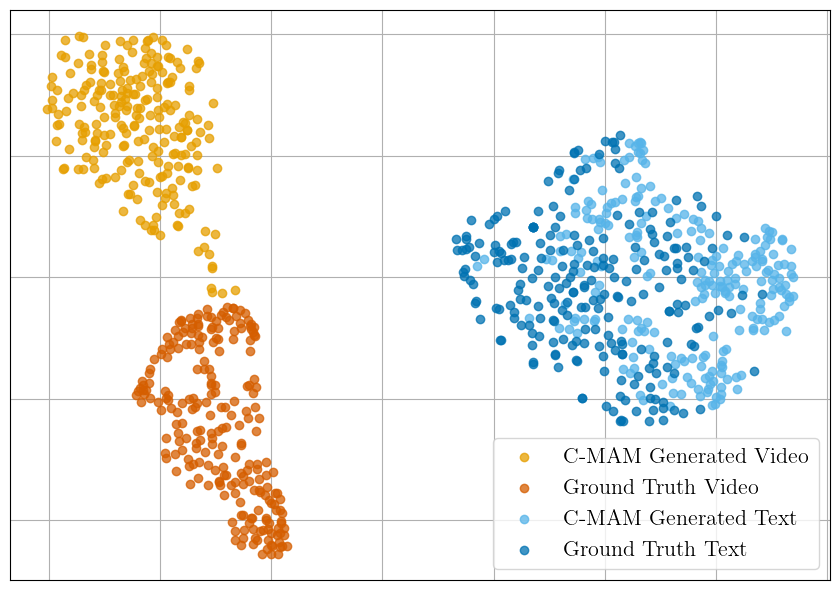
\includegraphics[width=\textwidth]{imgs/tsne/mmin/msp_improv/cmam_audio_tsne.png}
        \caption*{MSP-IMPROV (A $\rightarrow$ V+T)}
    \end{subfigure}
    \begin{subfigure}[b]{0.24\textwidth}
        \centering
        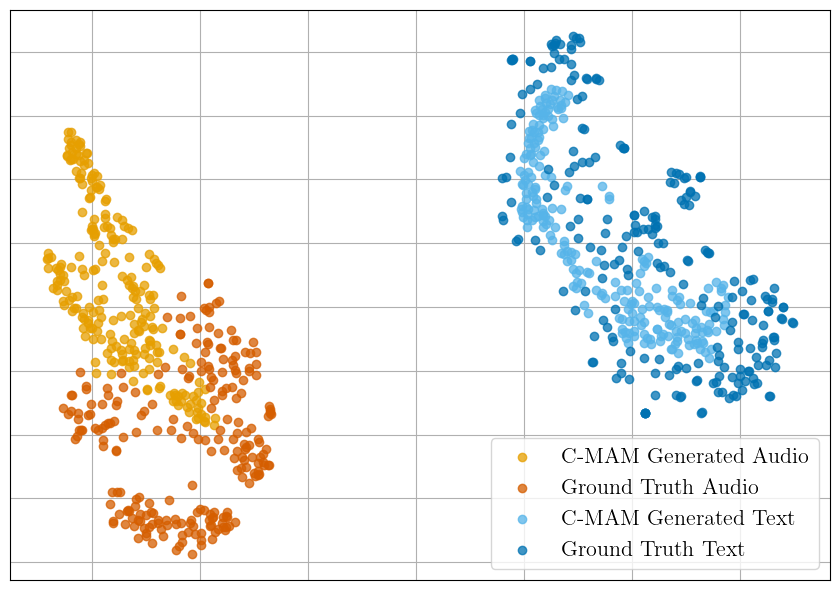
\includegraphics[width=\textwidth]{imgs/tsne/mmin/msp_improv/cmam_video_tsne.png}
        \caption*{MSP-IMPROV (V $\rightarrow$ A+T)}
    \end{subfigure}
    \begin{subfigure}[b]{0.24\textwidth}
        \centering
        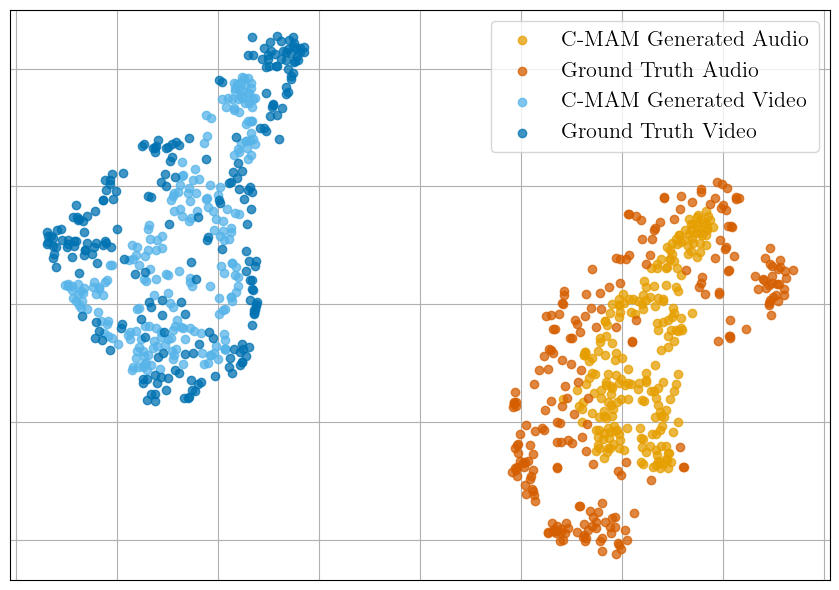
\includegraphics[width=\textwidth]{imgs/tsne/mmin/msp_improv/cmam_text_tsne.png}
        \caption*{MSP-IMPROV (T $\rightarrow$ A+L)}
    \end{subfigure}
    \begin{subfigure}[b]{0.24\textwidth}
        \centering
        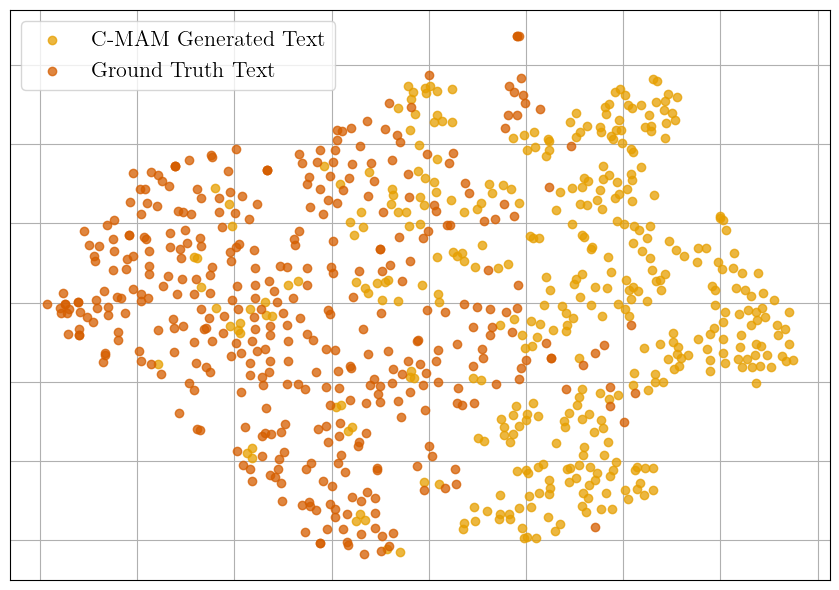
\includegraphics[width=\textwidth]{imgs/tsne/mmin/msp_improv/cmam_text_tsne_av.png}
        \caption*{MSP-IMPROV (AV $\rightarrow$ T)}
    \end{subfigure}
    \\
    \centering

    \begin{subfigure}[b]{0.24\textwidth}
        \centering
        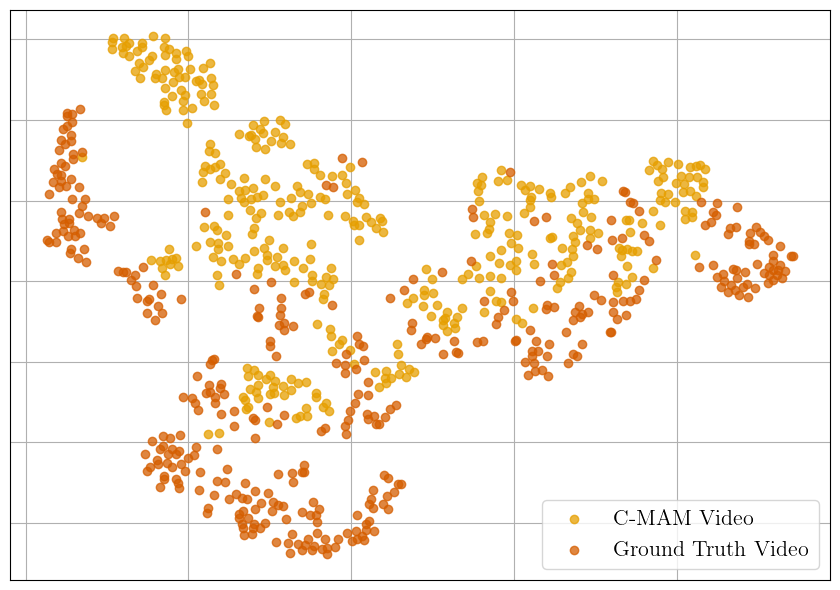
\includegraphics[width=\textwidth]{imgs/tsne/mmin/msp_improv/cmam_video_tsne_at.png}
        \caption*{MSP-IMPROV (AT $\rightarrow$ V)}
    \end{subfigure}
    \begin{subfigure}[b]{0.24\textwidth}
        \centering
        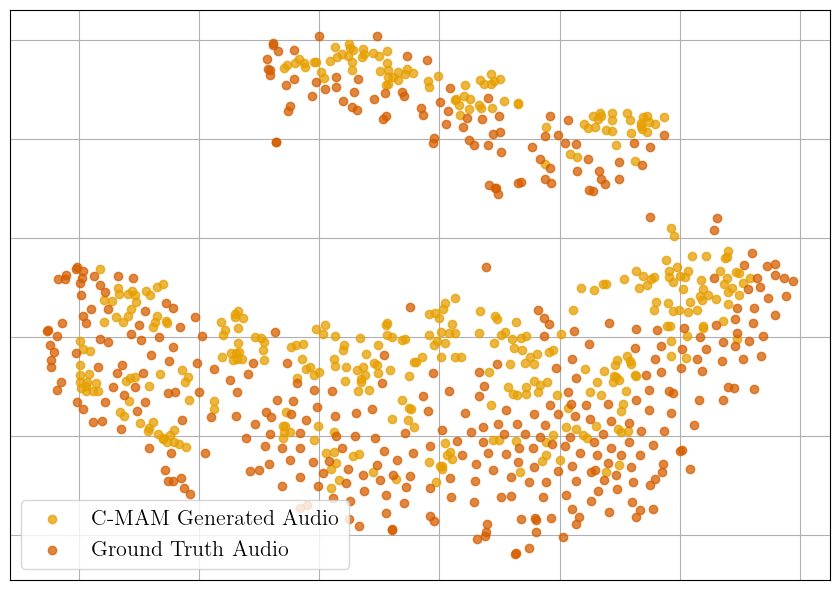
\includegraphics[width=\textwidth]{imgs/tsne/mmin/msp_improv/cmam_audio_tsne_vt.png}
        \caption*{MSP-IMPROV (VL $\rightarrow$ A)}
    \end{subfigure}
    \begin{subfigure}[b]{0.24\textwidth}
        \centering
        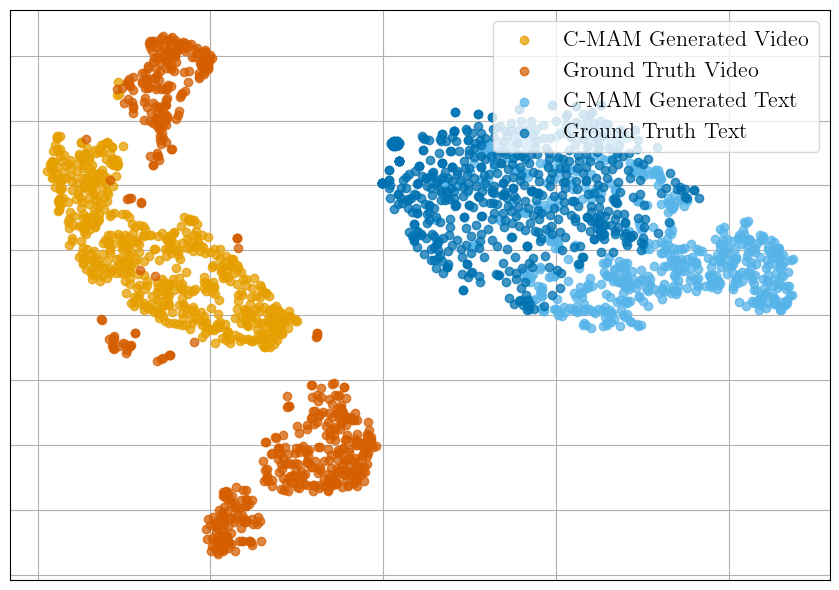
\includegraphics[width=\textwidth]{imgs/tsne/mmin/iemocap/cmam_audio_tsne.png}
        \caption*{IEMOCAP (A $\rightarrow$ V+T)}
    \end{subfigure}
    \begin{subfigure}[b]{0.24\textwidth}
        \centering
        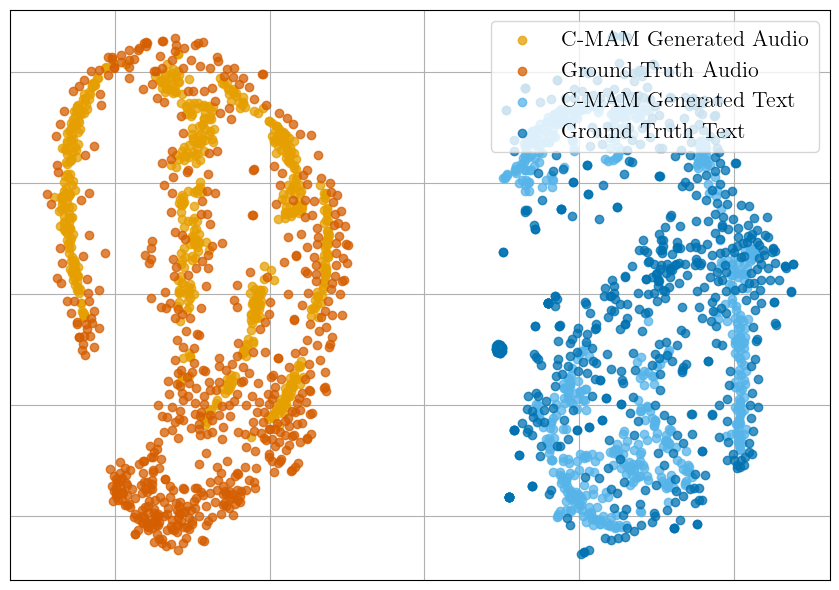
\includegraphics[width=\textwidth]{imgs/tsne/mmin/iemocap/cmam_video_tsne.png}
        \caption*{IEMOCAP (V $\rightarrow$ A+T)}
    \end{subfigure}
    \\
    \begin{subfigure}[b]{0.24\textwidth}
        \centering
        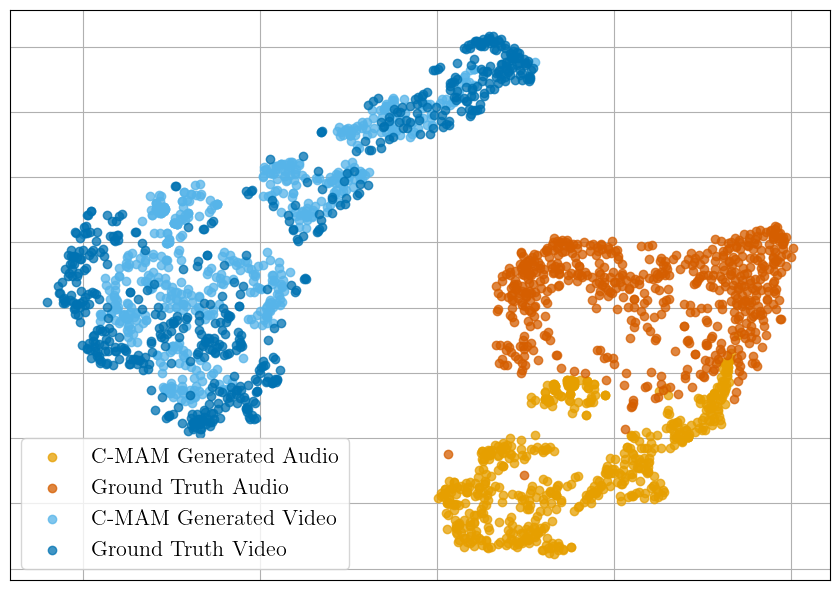
\includegraphics[width=\textwidth]{imgs/tsne/mmin/iemocap/cmam_text_tsne.png}
        \caption*{IEMOCAP (T $\rightarrow$ A+L)}
    \end{subfigure}
    \begin{subfigure}[b]{0.24\textwidth}
        \centering
        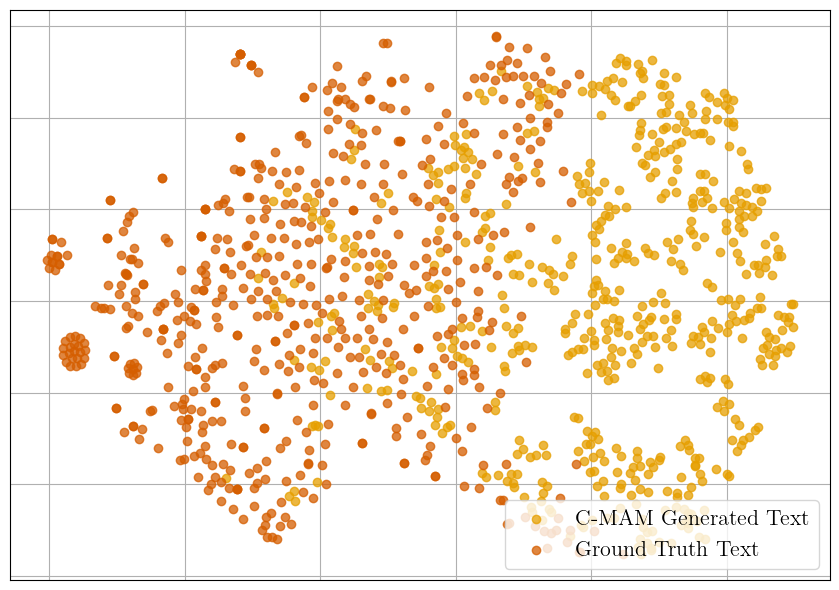
\includegraphics[width=\textwidth]{imgs/tsne/mmin/iemocap/cmam_gen_text_with_av.png}
        \caption*{IEMOCAP (AV $\rightarrow$ T)}
    \end{subfigure}
    \begin{subfigure}[b]{0.24\textwidth}
        \centering
        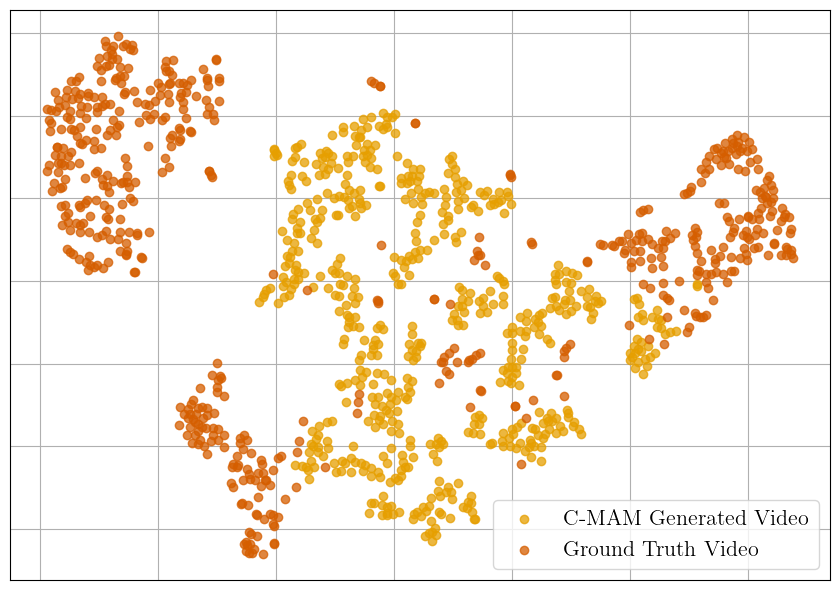
\includegraphics[width=\textwidth]{imgs/tsne/mmin/iemocap/cmam_gen_video_with_at.png}
        \caption*{IEMOCAP (AT $\rightarrow$ V)}
    \end{subfigure}
    \begin{subfigure}[b]{0.24\textwidth}
        \centering
        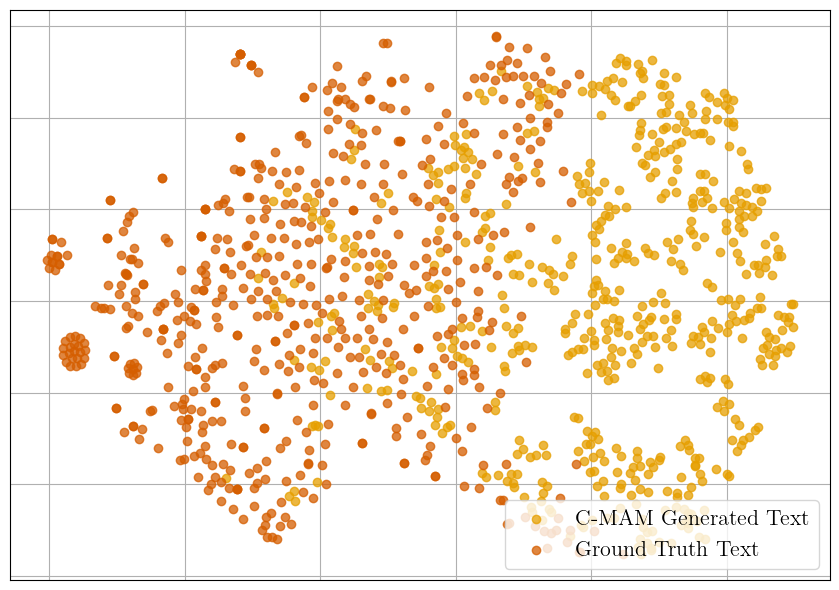
\includegraphics[width=\textwidth]{imgs/tsne/mmin/iemocap/cmam_gen_text_with_av.png}
        \caption*{IEMOCAP (VL $\rightarrow$ A)}
    \end{subfigure}
    \caption{T-SNE visualisations of the reconstructed embeddings vs. the ground truth features for each C-MAM trained.}
    \label{fig:tsne}

\end{figure}

% \end{landscape}

\textbf{C-MAM Reconstruction Error Metrics:} Table~\ref{tab:errors} presents reconstruction errors in terms of MAE and MSE for all the models tested in Section~\ref{sec:results}. Importantly, high reconstruction errors did not always correspond to poor performance recovery. This was particularly evident in the Kinetics-Sounds dataset, where despite significant reconstruction errors in the audio-to-video setting, C-MAMs still improved performance by 20\%-25\%. This suggests that the base multimodal model does not fully exploit all available modality information. C-MAMs can recover essential features even when the reconstructed embeddings are not exact replications of the ground truth. It also indicates how robust a multimodal model is to variances in the input data, as significant performance improvements were observed even when the reconstruction errors were high. The low error metrics demonstrate that C-MAMs effectively reconstruct missing modality embeddings.

\begin{table}[t!]
    \centering
    \caption{Error metrics between the ground truth feature embeddings produced by the trained modality-specific encoders and the C-MAM generated embeddings. Each row is organised as model - input modalities - output modality.}
    \label{tab:errors}
    \resizebox{\textwidth}{!}{%
    \begin{tabular}{l|cc|cc|l|cc}
    \hline
    \multirow{2}{*}{\textbf{Model \& C-MAM}}      & \multicolumn{2}{c|}{\textbf{IEMOCAP}} & \multicolumn{2}{c|}{\textbf{MSP-IMPROV}} & \multirow{2}{*}{\textbf{Model \& C-MAM}} & \multirow{2}{*}{\textbf{MAE}} & \multirow{2}{*}{\textbf{MSE}} \\ \cline{2-5}
                                                  & \textbf{MSE}      & \textbf{MSE}      & \textbf{MAE}        & \textbf{MSE}       &                                          &                               &                               \\ \hline
    \textbf{MMIN - Audio - Video}                 & 0.2205            & 0.1073            & 0.2106              & 0.0740             & \textbf{Audioset - Audio - Video}        & 0.3297                        & 0.1849                        \\
    \textbf{MMIN - Audio - Text}                  & 0.2272            & 0.1915            & 0.2691              & 0.3321             & \textbf{AudioSet - Video - Audio}        & 0.3804                        & 0.2190                        \\ \cline{6-8} 
    \textbf{MMIN - Audio/Video - Text}            & 0.2553            & 0.2387            & 0.2727              & 0.4158             & \textbf{AVMNIST - Audio - Image}         & 1.1611                        & 2.7552                        \\
    \textbf{MMIN - Audio/Text - Video}            & 0.0673            & 0.0089            & 0.0899              & 0.1413             & \textbf{AVMNIST - Image - Audio}         & 0.6106                        & 0.6121                        \\ \cline{6-8} 
    \textbf{MMIN - Video - Audio}                 & 0.0399            & 0.1558            & 0.2601              & 0.1158             & \textbf{Kinetics-Sounds - Audio - Video} & 3.8226                        & 32.7867                       \\
    \textbf{MMIN - Video - Text}                  & 0.2127            & 0.1955            & 0.1272              & 0.1825             & \textbf{Kinetics-Sounds - Video - Audio} & 0.6905                        & 1.3158                        \\ \cline{6-8} 
    \textbf{MMIN - Video/Text - Audio}            & 0.1044            & 0.0179            & 0.1282              & 0.0271             & \textbf{MM-IMDb - Image - Text}          & 0.2962                        & 0.1627                        \\
    \textbf{MMIN - Text - Audio}                  & 0.1917            & 0.0658            & 0.1547              & 0.0382             & \textbf{MM-IMDb - Text - Image}          & 0.2901                        & 0.1417                        \\
    \textbf{MMIN - Text - Video}                  & 0.0534            & 0.0071            & 0.0806              & 0.0133             &                                          &                               &                               \\ \cline{1-5}
    \textbf{}                                     & \multicolumn{2}{c|}{\textbf{MOSI}}    & \multicolumn{2}{c|}{\textbf{MOSEI}}      &                                          &                               &                               \\ \cline{1-5}
    \textbf{EMT-DLFR - Audio/Video - Text}        & 0.3461            & 0.2014            & 0.2690              & 0.1347             &                                          &                               &                               \\
    \textbf{Robust EMT-DLFR - Audio/Video - Text} & 0.3162            & 0.1886            & 0.3092              & 0.1657             &                                          & \multicolumn{1}{l}{}          & \multicolumn{1}{l}{}          \\ \hline
    \end{tabular}%
    }
\end{table}

\textbf{Statistical Analysis:} A detailed statistical analysis was conducted to quantify the alignment between reconstructed and ground-truth embeddings for the MM-IMDb, and MOSEI datasets. This analysis employed three complementary approaches: cosine similarity distributions to assess directional alignment, dimension-wise effect sizes to measure the magnitude of differences, and statistical significance tests to evaluate the reliability of these differences. Each dataset revealed distinct patterns in how C-MAMs preserve structural relationships in the latent space.

\begin{figure}[b!]
    \centering
    \includegraphics[width=0.875\textwidth]{imgs/MMIMDB/image_to_text/statstical_analysis.pdf}
    \includegraphics[width=0.875\textwidth]{imgs/MMIMDB/text_to_image/statstical_analysis.pdf}
    \caption{Statistical analysis of C-MAMs' reconstruction quality for the MM-IMDb dataset. The analysis includes a cosine similarity distribution, dimension-wise effect size analysis, and a volcano plot for mean difference significance.}
    \label{fig:mmimdb_stats}
\end{figure}

The \textbf{MM-IMDb} dataset and model presented a more nuanced picture of reconstruction effectiveness (see \Cref{fig:mmimdb_stats}). Despite showing relatively low directional alignment, with the Text-to-Image case exhibiting a mean cosine similarity of 0.051, C-MAMs enabled near-baseline performance recovery. This apparent contradiction prompted a dedicated sub-ablation study investigating whether explicitly optimising for directional alignment via cosine similarity loss would improve performance. The results, presented in Table~\ref{tab:mmimdb_sub_ablation}, revealed that neither pure cosine similarity loss nor a combined MSE and cosine similarity loss significantly improved reconstruction quality or performance metrics. This finding suggests that the multimodal model exhibits robustness to deviations in latent space alignment, with perfect cosine similarity not being a prerequisite for effective downstream classification.

\begin{table}[tb]
    \centering
    \caption{analysis of how varying the cosine loss term influences model performance metrics and embedding reconstruction in the MM-IMDb multimodal dataset.}
    \label{tab:mmimdb_sub_ablation}
    \resizebox{\textwidth}{!}{%
    \begin{tabular}{l|ccccc|ccccc}
    \hline
                            & \multicolumn{5}{c|}{\textbf{Image $\mapsto$ Text}}                                                      & \multicolumn{5}{c}{\textbf{Text $\mapsto$ Image}}                                                       \\ \cline{2-11} 
                            & \textbf{F1-Weighted} & \textbf{F1-Samples} & \textbf{F1-Micro} & \textbf{F1-Macro} & \textbf{Cos. Sim.} & \textbf{F1-Weighted} & \textbf{F1-Samples} & \textbf{F1-Micro} & \textbf{F1-Macro} & \textbf{Cos. Sim.} \\ \hline
    \textbf{MSE}            & 0.4019               & 0.4489              & 0.4577            & 0.2282            & 0.0974             & 0.5743               & 0.5986              & 0.6015            & 0.4232            & 0.0512             \\
    \textbf{Cos. Sim.}      & 0.4266               & 0.4302              & 0.4362            & 0.2695            & 0.1704             & 0.5148               & 0.5076              & 0.5128            & 0.3871            & 0.1430             \\
    \textbf{MSE + Cos. Sim} & 0.43088              & 0.4570              & 0.4658            & 0.2608            & 0.1556             & 0.5715               & 0.5877              & 0.5904            & 0.236             & 0.1253             \\ \hline
    \end{tabular}%
    }
\end{table}

\begin{figure}[pb!]
    \centering
    \includegraphics[width=0.875\textwidth]{imgs/MOSEI/audio_to_text/statstical_analysis.pdf}
    \includegraphics[width=0.875\textwidth]{imgs/MOSEI/audio_text_to_video/statstical_analysis.pdf}
    \caption{Statistical analysis of C-MAMs' reconstruction quality across a selection of missing conditions for the MOSEI dataset. Each includes a cosine similarity distribution, dimension-wise effect size analysis, and a volcano plot for mean difference significance. The remaining missing modality conditions are presented in the appendices.}
    \label{fig:mosei_stats}
\end{figure}

The \textbf{MOSEI} dataset analysis\footnote{See Section~\ref{sec:MOSEI} of the appendices for the analysis on all missing modality conditions trained the Utterance Fusion model \cite{zhao-etal-2021-missing} using the MOSEI dataset.} (see Figure~\ref{fig:mosei_stats}) revealed varying patterns across different modality combinations, providing insights into the relationship between reconstruction quality and model performance. The Audio-to-Text condition demonstrated strong directional alignment with right-skewed cosine similarity distributions. However, the volcano plot analysis revealed that many dimensions still exhibited statistically significant differences, despite effect sizes being near zero. The Audio and Text-to-Video condition showed moderately strong alignment with a mean cosine similarity of 0.78 and median of 0.80. However, effect size analysis indicated the presence of small but statistically significant deviations. These patterns suggest that while C-MAMs achieve strong overall latent space alignment, the presence of small dimensional deviations does not impact downstream performance significantly.

The collective findings from this statistical analysis reveal three key insights about C-MAM behaviour. First, the degree of embedding alignment achieved by C-MAMs varies across datasets and modality combinations, suggesting that different modality pairs may require different levels of reconstruction precision. Second, strong performance improvements can be achieved even with imperfect reconstruction, indicating that multimodal models are robust to certain embedding deviations. Third, statistically significant dimensional differences do not necessarily correspond to degraded performance, suggesting that some embedding dimensions may be redundant or non-critical for the downstream task. These insights validate the effectiveness of C-MAMs and guide future optimisation of missing modality reconstruction techniques.

\textbf{Contrastive Information in Learned Embeddings: } Multimodal learning is often assumed to benefit from mutual and complementary information across modalities. However, our analysis reveals that modality-specific encoders do not always preserve these relationships, as \textit{contrastive embeddings} can emerge during training. In such cases, embeddings from different modalities become misaligned in feature space, which can reduce their informativeness when combined. The impact on downstream performance depends on the extent of contrastiveness, the nature of the task, and whether the fusion and classification layers compensate for misaligned features.

To better understand this, we analysed learned modality embeddings across AVMNIST, Kinetics-Sounds, and MOSEI. Kinetics-Sounds exhibited the strongest contrastive behaviour, with high KL divergence and near-zero cosine similarity between audio and video embeddings, indicating that the model disregarded audio features entirely. MOSEI showed moderate contrastiveness, where the dominance of text led to weaker reliance on audio and video. In AVMNIST, contrastive embeddings were present, yet performance remained unaffected. This demonstrates that contrastiveness does not always degrade results. Even misaligned embeddings can still support accurate reconstruction when a task is highly redundant, as in digit classification.

Contrastive embeddings are not necessarily an inherent dataset property but can emerge due to the training dynamics of modality-specific encoders. While contrastiveness can impact missing modality reconstruction, its effect depends on whether the fusion mechanism and classifier can compensate for the misalignment. In AVMNIST, the classifier extracted class-relevant features despite embeddings being nearly orthogonal, allowing C-MAMs to achieve full performance recovery. In contrast, Kinetics-Sounds showed that when contrastiveness is severe and fusion cannot realign features, one modality may be ignored, leading to degraded performance when it is missing.

Despite evidence of contrastive embeddings across all datasets, \textbf{C-MAMs remained highly effective in recovering missing modality performance}. Their ability to restore meaningful information, even in contrastive settings, suggests that contrastive embeddings do not always prevent reconstruction but may introduce additional challenges depending on how well learned features align. Further details and statistical analyses are provided in Appendix~\ref{sec:contrastive_info}.

\textbf{C-MAM Data Requirements:} A key consideration in the post-training C-MAM approach is the requirement to train new C-MAMs on the full dataset, which can be computationally expensive. We conduct experiments using progressively larger balanced subsets (10\%-100\%) of AVMNIST, MM-IMDb, and MOSEI to assess the minimum training data necessary, evaluating C-MAMs on the full test set. The results show that \textbf{C-MAMs trained with as little as 10\% of the data achieve strong performance}, with only minor differences from full dataset training. Larger datasets lead to faster convergence but not necessarily better final performance, suggesting that \textit{learnt latent spaces remain robust} even with limited training. In MM-IMDb, stronger modality dependence causes greater instability at lower data availability, though test performance remains stable. In MOSEI, text-based conditions are largely unaffected by training size, reinforcing the \textit{importance of modality-specific learning dynamics}.

These findings highlight the \textit{efficiency of learning a static latent space post-training}, which remains transferable across different training conditions. Full experimental results are provided in the appendix.

\textbf{Observability into Multimodal Model Performance:} This work emphasises detailed evaluation of missing modality conditions, an often-overlooked aspect of multimodal learning. Many studies assess robustness in aggregate, neglecting how missing modalities impact latent space structure and performance. Our experiments show that even with low cosine similarity between reconstructed and ground-truth embeddings, C-MAMs can still recover task performance. This is especially evident in MM-IMDb, where Text-to-Image reconstruction yielded low similarity yet restored F1 scores to the baselines. These findings highlight the need for task-aware evaluations over standard embedding similarity metrics. Beyond performance reporting, we provide embedding visualisations, statistical significance tests, and effect size analyses, revealing that statistically significant deviations in individual dimensions do not necessarily harm inference. Future work should explore whether these insights generalise across architectures and whether tools like SHAP or saliency maps could enhance interpretability. As multimodal models see real-world deployment, a standardised missing modality evaluation framework is crucial. Our results suggest comprehensive error analysis, visualisation techniques, and task-aware evaluations are essential for assessing robustness to missing data.


\textbf{Limitations and Future Directions:} While C-MAMs offer a modular solution for missing modality reconstruction, their effectiveness \textbf{depends on the base multimodal model's learned representations}. Reconstruction may have limited impact if a modality is underutilised during training, making C-MAMs ineffective in addressing inherent modality imbalances. \textbf{Scalability} remains a challenge, as the number of required C-MAMs grows exponentially (the total can be expressed as $2^K - 2$) with the number of modalities. Training separate models for each missing modality scenario increases computational overhead. Research into multimodal reconstruction strategies that generalise across missing conditions without sacrificing specificity could improve efficiency. However, given the strong performance of the current approach, additional complexity should be introduced only where meaningful gains are observed. C-MAMs also require \textbf{access to the original dataset} for training, which may pose challenges in privacy-sensitive applications and requires an investigation into training C-MAMs using privacy-preserving techniques and minimal amounts of data. Furthermore, while MSE has proven effective, it does not explicitly enforce semantic consistency. Future work could explore alternative loss functions, such as contrastive learning, to improve reconstruction alignment. 

Beyond these technical improvements, future work should also establish standardised evaluation frameworks for missing modality reconstruction, considering both reconstruction quality and downstream task performance. Addressing these limitations while preserving simplicity and flexibility will be key to ensuring broader applicability as multimodal systems expand.
